\documentclass[]{article}
\usepackage{listings} 
\usepackage{algorithm}
\usepackage{algorithmic}
\usepackage{graphicx}
\graphicspath{ {images/} }
\usepackage{float}
\usepackage{geometry}
\usepackage{pdfpages}

%opening
\title{}
\author{}
\date{}
\special{papersize=8.5in,11in}
\geometry{left=1.5cm,right=2cm,top=1.5cm,bottom=1.5cm}

\begin{document}
	
	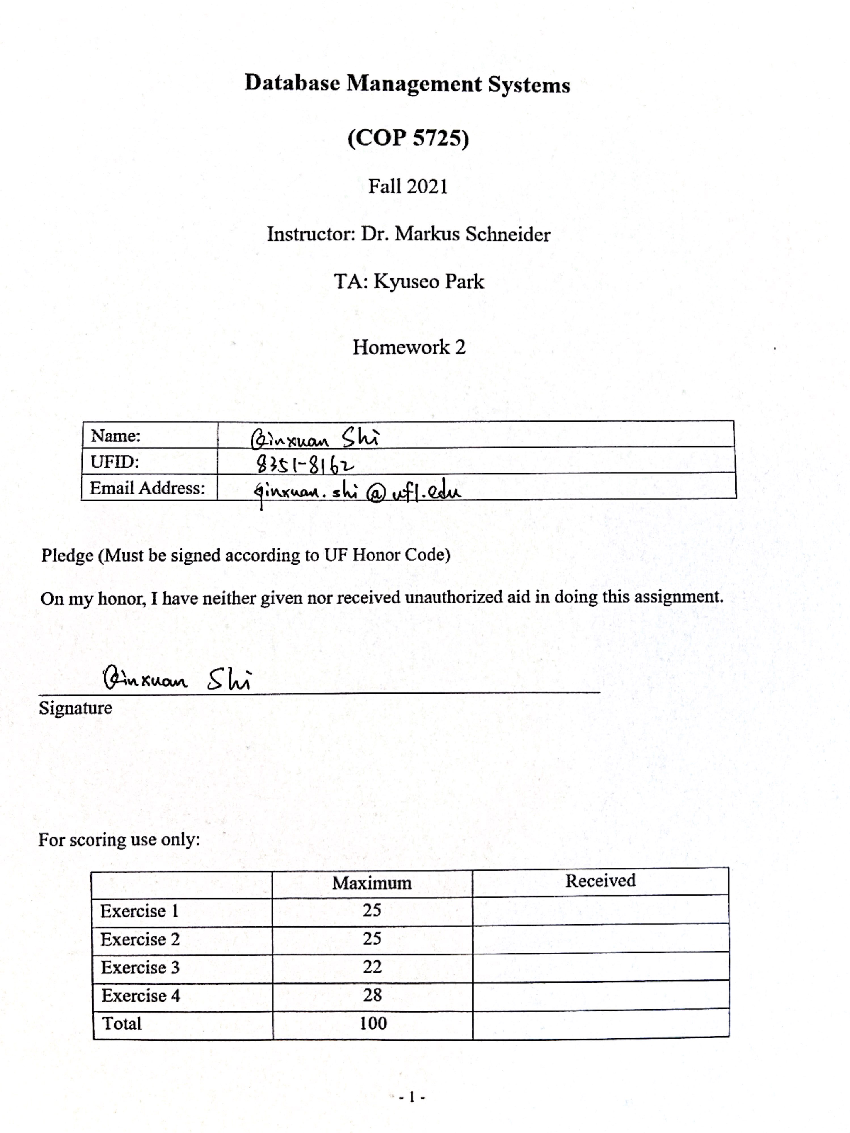
\includepdf{./document-H1/Homework2.pdf}
	
	\section{Exercise 1}
	
	\noindent(1) Find the names of IT department employees who do not work on any project that the IT department runs.\\

	IT department employees:\\
	
	$Employee\_IT\leftarrow \rho_{Employee\_IT}(\pi_{(SSN,name)}(Employee\bowtie_{Employee.Dno=Department.Dnumber\wedge Department.name='IT'} Department))$
	\\
	
	projects that the IT department runs:\\	

	$Project\_IT\leftarrow \rho_{Project\_IT}(\pi_{Pnumber}(Project\bowtie_{Project.Dno=Department.Dnumber\wedge Department.name='IT'} Department))$\\
	
	Employee who work on the projects that the IT department runs:\\
	
	$Employee\_Project\_IT\leftarrow \rho_{Employee\_Project\_IT}(\pi_{Essn}(Works\_on\bowtie_{Pno=Pnumber} Project\_IT))$\\
	
	the names of IT department employees who do not work on any project that the IT department runs:\\
	
	$\pi_{name}(Employee\_IT)- \pi_{name}(Employee\_IT\bowtie_{SSN=Essn} Employee\_Project\_IT)$\\
	
	\noindent(2) Find the names of departments that are located at the same location as the IT department.\\
	
	join department with its location:\\
	
	$D\leftarrow \rho_{D}(Department\bowtie Dept\_location)$\\
	
	$D_{1}\leftarrow \rho_{D_{1}}(D)$\\
	
	$D_{2}\leftarrow \rho_{D_{2}}(D)$\\
	
	get the names of departments that are located at the same location as IT department ('IT' is not included):\\
	
	$\pi_{D_{2}.name}(D_{1}\bowtie_{D_{1}.Dlocation=D_{2}.Dlocation\wedge D_{1}.name='IT'\wedge D_{2}.name\neq'IT'} D_{2})$\\
	
	\noindent(3) Find the names of employees who work the most hours on projects that the IT 
	department runs.\\
	
	projects that the IT department runs:\\	
	
	$Project\_IT\leftarrow \rho_{Project\_IT}(\pi_{Pnumber}(Project\bowtie_{Project.Dno=Department.Dnumber\wedge Department.name='IT'} Department))$\\
	
	Employee who work on the projects that the IT department runs:\\
	
	$E\leftarrow \rho_{E}(Works\_on\bowtie_{Woks\_on.Pno=Project\_IT.Pnumber} Project\_IT)$\\
	
	$E_{1}\leftarrow \rho_{E_{1}}(E)$\\
	
	$E_{2}\leftarrow \rho_{E_{2}}(E)$\\
	
	get names of employees who work the most hours:\\
	
	$\pi_{name}((\pi_{Essn}(E)-\pi_{E_{2}.Essn}(E_{1}\bowtie_{E_{1}.hours>E_{2}.hours}E_{2}))\bowtie_{Essn=SSN} Employee)$\\
	
	\noindent(4) Find the names of employees who work on both Project ‘A’ and Project ‘B’.\\
	
	employees who work on Project 'A':\\
	
	$E\_P_{A}\leftarrow \rho_{E\_P_{A}}(\pi_{Essn}(Project\bowtie_{Project.Pnumber=Works\_on.Pno\wedge Project.name='A'} Works\_on))$\\
	
	employees who work on Project 'B':\\
	
	$E\_P_{B}\leftarrow \rho_{E\_P_{B}}(\pi_{Essn}(Project\bowtie_{Project.Pnumber=Works\_on.Pno\wedge Project.name='B'} Works\_on))$\\
	
	names of employees who work on both:\\
	
	$\pi_{name}(Employee\bowtie_{SSN=Essn}(E\_P_{A}\cap E\_P_{B}))$\\
	
	\noindent(5) Find the name of employees who work on every project run by the IT department.\\
	
	projects run by the IT department, rename Pnumber to Pno:\\
	
	$E\_IT\leftarrow \rho_{E\_IT}(\pi_{Pnumber}(Project\bowtie_{Project.Dno=Department.Dnumber\wedge Department.name='IT'} Department))$\\
	
	$\rho_{Pno\leftarrow Pnumber}(E\_IT)$\\
	
	divide all projects, get the name of employees:\\
	
	$\pi_{name}((\pi_{Essn}(Works\_on\div E\_IT))\bowtie_{Essn=SSN} Employee)$\\
	
	
	\clearpage
	\section{Exercise 2}
	
	\noindent(1)  Find the names of customers who have booked flights at every company in the US.\\
	
	$\pi_{name}((\pi_{customer\_ID}(Book\div \pi_{company\_ID}(\sigma_{location='US'}(Company))))\bowtie Customer)$\\
	
	\noindent(2) Find the names of customers who have never booked a flight.\\
	
	$\pi_{name}((\pi_{customer\_ID}(Customer)- \pi_{customer\_ID}(Book))\bowtie Customer)$\\

	\noindent(3) Find the names of customers who booked the flight to New York more than once.\\
	
	customers who booked the flight to New York:\\
	
	$C\leftarrow \rho_{C}(\pi_{(company\_ID,flight\_number,customer\_ID)}(\sigma_{Flight.destination='New York'}(Book\bowtie Flight)))$\\
	
	$C_{1}\leftarrow \rho_{C_{1}}(C)$\\
	
	$C_{2}\leftarrow \rho_{C_{2}}(C)$\\
	
	two flights are booked by the same customer with different company\_ID OR different flight\_number:\\
	
	$\rho_{C\_id}(\pi_{C_{1}.customer\_ID}(C_{1}\bowtie_{C_{1}.customer\_ID=C_{2}.customer\_ID\wedge(C_{1}.flight\_number\neq C_{2}.flight\_number\vee C_{1}.company\_ID\neq C_{2}.company\_ID)} C_{2}))$\\
	
	$\pi_{name}(C\_id\bowtie Customer)$\\
	
	\noindent(4) Find the names of the companies that have the biggest (in terms of the number of 
	seats) airplane.\\
	
	$F_{1}\leftarrow \rho_{F_{1}}(Flight)$\\
	
	$F_{2}\leftarrow \rho_{F_{2}}(Flight)$\\
	
	get company\_ID and flight\_number of the biggest airplane:\\ 
	
	$B\leftarrow \rho_{B}(\pi_{(company\_ID,flight\_number)}(Flight)-\pi_{(F_{2}.company\_ID,F_{2}.flight\_number)}(F_{1}\bowtie_{F_{1}.number\_of\_seats>F_{2}.number\_of\_seats}F_{2}))$\\
	
	$\pi_{company\_name}(Company\bowtie B)$\\
	
	\noindent(5) Find the names of customers who booked flights to Boston and Seattle.\\
	
	$\pi_{name}(((\pi_{customer\_ID}(\sigma_{Flight.destination='Boston'}(Book\bowtie Flight)))\cap(\pi_{customer\_ID}(\sigma_{Flight.destination='Seattle'}(Book\bowtie Flight))))\bowtie Customer)$\\
	
	\noindent(6) Find all destinations (unequal to Gainesville) of cheap flights (<=500) provided 
	by companies that also provide flights to Gainesville.\\
	
	get the flights provided by companies that provide flights to Gainesville:\\
	
	$Fc\leftarrow \rho_{Fc}((\pi_{company\_ID}(\sigma_{destination='Gainesville'}(Flight)))\bowtie Flight)$\\
	
	get destinations of flights have cheap prices:\\
	
	$\pi_{destination}(\sigma_{price<=500\wedge destination\neq'Gainesville'}(Fc))$\\
	
	\clearpage
	\section{Exercise 3}
	
	\noindent(1) Find the names and GPA of CISE students who have enrolled in the DB class.\\
	
	get the students who enrolled in DB class:\\
	
	$S\_DB\leftarrow \rho_{S\_DB}(\pi_{student\_ID}((\pi_{class\_ID}(\sigma_{name='DB'}(Class)))\bowtie Enroll))$\\
	
	get the names and gpa of CISE students:\\
	
	$\pi_{(name,gpa)}(\sigma_{major='CISE'}(S\_DB\bowtie Student))$\\
	
	\noindent(2) Find the names and major of students who have enrolled in the DB class on 
	Wednesdays and the Algorithm class on Thursdays but have not enrolled in the OS class on 
	Fridays.\\
	
	students who enrolled in the DB class on Wednesday:\\
	
	$S_{DB}\leftarrow \rho_{S_{DB}}(\pi_{student\_ID}((\pi_{class\_ID}(\sigma_{name='DB'\wedge day='Wednesday'}(Class)))\bowtie Enroll))$\\
	
	students who enrolled in the Algorithm class on Thursday:\\
	
	$S_{A}\leftarrow \rho_{S_{A}}(\pi_{student\_ID}((\pi_{class\_ID}(\sigma_{name='Algorithm'\wedge day='Thursday'}(Class)))\bowtie Enroll))$\\
	
	students who enrolled in the OS class on Friday:\\
	
	$S_{OS}\leftarrow \rho_{S_{OS}}(\pi_{student\_ID}((\pi_{class\_ID}(\sigma_{name='OS'\wedge day='Friday'}(Class)))\bowtie Enroll))$\\
	
	get the results:\\
	
	$\pi_{(name,major)}((S_{DB}\cap S_{A}\cap(\pi_{student\_ID}(Student)-S_{OS}))\bowtie Students)$\\
	
	\noindent(3) Find the names and major of students who have enrolled in every class taught by 
	‘James’.\\
	
	students who enrolled in all class taught by 'James':\\
	
	$S_{J}\leftarrow \rho_{S_{J}}(\pi_{student\_ID}(Enroll\div\pi_{class\_ID}(\sigma_{lecturer='James'}(Class))))$\\
	
	get the results:\\
	
	$\pi_{(name,major)}(S_{J}\bowtie Students)$\\
	
	\noindent(4) Find the names of students who have enrolled in the DB class more than twice.\\
	
	students who enrolled in the DB class:\\
	
	$E\leftarrow \rho_{E}(\pi_{(student\_ID,semester)}((\pi_{class\_ID}(\sigma_{name='DB'}(Class)))\bowtie Enroll))$\\
	
	$E_{1}\leftarrow \rho_{E_{1}}(E)$\\
	
	$E_{2}\leftarrow \rho_{E_{2}}(E)$\\
	
	$E_{3}\leftarrow \rho_{E_{3}}(E)$\\
	
	the records of the same student:\\
	
	$T\leftarrow \rho_{T}(\sigma_{E_{1}.student\_ID=E_{2}.student\_ID\wedge E_{2}.student\_ID=E_{3}.student\_ID}(E_{1}\times E_{2}\times E_{3}))$\\
	
	three semester are all different, get the results:\\
	
	$\pi_{name}((\pi_{E_{1}.student\_ID}(\sigma_{E_{1}.semester\neq E_{2}.semester\wedge E_{2}.semester\neq E_{3}.semester\wedge E_{1}.semester\neq E_{3}.semester}(T)))\bowtie Students)$\\
	
	\noindent(5) Find the names of students who have not enrolled in the DB class.\\

	students who enrolled in the DB class:\\
	
	$S_{DB}\leftarrow \rho_{S_{DB}}(\pi_{student\_ID}((\pi_{class\_ID}(\sigma_{name='DB'}(Class)))\bowtie Enroll))$\\
	
	get the results:\\
	
	$\pi_{name}((\pi_{student\_ID}(Student)-S_{DB})\bowtie Students)$\\
	
	\clearpage
	\section{Exercise 4}
	
	\noindent 1. The term is not correct in general. Only when $A_{1}\sqsubseteq A_{2}\sqsubseteq A_{3}...\sqsubseteq A_{n}$ the statement is true.\\
	
	\noindent Proof: \\
	
	\noindent We assume that the relation R have the schema $R(X_{1}:D_{1},X_{2}:D_{2},...,X_{3}:D_{n})$, let two subsets $A_{i}$ and $A_{j}$($\exists i,j, 1\le i,j\le n $ and $i<j$). Assume that $A_{i}$ has several attributes, $A_{i}(X_{a}, X_{b}, X_{c}...)$ and $A_{j}$ also have several attributes $A_{j}(X_{x}, X_{y}, X_{z}...)$. Then we consider about the statement $\pi_{A_{i}}(\pi_{A_{j}}(R)) = \pi_{A_{i}}(R)$.\\
	
	\noindent Since all of the attributes of $A_{j}$ are contained in $R$, so the result $R'$ of $\pi_{A_{j}}(R)$ is the same schema as $A_{j}$, then we have $\pi_{A_{i}}(R')$. However, there might be different results according to the relation between $A_{i}$ and $A_{j}$.\\
	
	(1) if all of the attributes of $A_{i}$ are not contained in $A_{j}$, it is obvious that $\pi_{A_{i}}(R') = \emptyset$. So the statement won't be true.\\
	
	(2) if some of the attributes of $A_{i}$ are not contained in $A_{j}$, it is also obvious that there won't be any results for $\pi_{A_{i}}(R')$. So the statement is not true.\\
	
	(3) if all of the attributes of $A_{i}$ are contained in $A_{j}$, then the result of $\pi_{A_{i}}(R')$: $R''$  has the same schema as $\pi_{A_{i}}(R)$. So the statement is true.\\
	
	\noindent To conclude, only when all of the attributes of $A_{i}$ are contained in $A_{j}$, which is $A_{i}\sqsubseteq A_{j}$, then $\pi_{A_{i}}(\pi_{A_{j}}(R)) = \pi_{A_{i}}(R)$.\\
	
	\noindent It is also the same when we consider the term of the problem, only when $A_{i}$ is contained by $A_{j}$, for $\forall i,j, 1\le i<j\le n$, which is $A_{1}\sqsubseteq A_{2}\sqsubseteq A_{3}...\sqsubseteq A_{n}$, then the term will be true.\\
	
	
	\noindent 2. Only when all of the attribute names contained in $F$ are also contain in $A$, the statement is true.\\
	
	\noindent Proof: \\
	
	\noindent We assume that relation A has the schema $A(A_{i},..., A_{j})$, in which $\forall i,j, 1\le i<j\le n$, and the set of attributes which names are involved in F: $B(A_{k}, A_{l}...)$.\\
	
	(1) if all of the attributes in B are not included in A, then there will be no result for $\sigma_{F}(\pi_{A}(R))$. \\
	
	(2) if some of the attributes in B are not included in A, then there will also be no result for $\sigma_{F}(\pi_{A}(R))$. \\
	
	(3) if all of the attributes in B are included in A, then the schema of $\sigma_{F}(\pi_{A}(R))$ and $\pi_{A}(\sigma_{F}(R))$ will be the same. What's more, since all of the attribute name in F are contained in A, there is no difference in tuples between them.\\
	
	\noindent To conclude, only when all of the attribute names contained in $F$ are also contain in $A$, the statement is true.\\
	
	\noindent 3. a. We consider $R(A, B)\cup T(A, B)$\\
	
	Maximum: when R and T don't have duplicate tuples, which is $R\cap T=\emptyset$, then the number is r+s.\\
	
	Minimum:\\
	
	(1) $R=T$, then the result is r, s;\\
	
	(2) $R\sqsubseteq T$, then the result is s;\\
	
	(3) $T\sqsubseteq R$, then the result is r;\\
	
	As a result, the minimum number of tuples is $max(r, s)$.\\
	
	\noindent b. Exactly, $R\bowtie R=R$, then we can know $R\bowtie(R\bowtie R)=R$. \\
	
	To conclude, Minimum is r and Maxmum is also r.\\
	
	\noindent c. To consider $\pi_{A, C}(R\bowtie S)$, we can consider the result of $R\bowtie S$. \\
	
	Maximum: when all the values of B in either R and S are same, which means $\vert\pi_{B}(R)\vert=\vert\pi_{B}(S)\vert=1$, then $\vert R\bowtie S\vert$ will be the maximum, so the maximum number is $r\cdot s$.\\
	
	Minimum: when $R\bowtie S=\emptyset$. there will be no result for projection, so the minimum is 0.\\
	
	\noindent d. To consider $\sigma_{A=C}(R\bowtie S)$, we can also consider the result of $R\bowtie S$. \\
	
	Maximum: when all the values of B in either R and S are same, which means $\vert\pi_{B}(R)\vert=\vert\pi_{B}(S)\vert=1$, then the maximum number is depend on the minimum of $\vert\pi_{A}(R)\vert$ and $\vert\pi_{C}(S)\vert$. As a result, the maximum number is $min(r, s)$.\\
	
	Minimum: \\
	
	(1) when $R\bowtie S=\emptyset$, there will be no result for projection, so the minimum is 0.\\
	
	(2) There is another situation, although $R\bowtie S\neq\emptyset$, there is no tuple $A=C$.\\
	
	To conclude, the minimum number is 0.
	
	
\end{document}
